\documentclass[12pt, twoside]{article}
\usepackage[letterpaper, margin=1in, headsep=0.2in]{geometry}
\setlength{\headheight}{0.6in}
%\usepackage[english]{babel}
\usepackage[utf8]{inputenc}
\usepackage{microtype}
\usepackage{amsmath}
\usepackage{amssymb}
%\usepackage{amsfonts}
\usepackage{siunitx} %units in math. eg 20\milli\meter
\usepackage{yhmath} % for arcs, overparenth command
\usepackage{tikz} %graphics
\usetikzlibrary{quotes, angles}
\usepackage{graphicx} %consider setting \graphicspath{{images/}}
\usepackage{parskip} %no paragraph indent
\usepackage{enumitem}
\usepackage{multicol}
\usepackage{venndiagram}

\usepackage{fancyhdr}
\pagestyle{fancy}
\fancyhf{}
\renewcommand{\headrulewidth}{0pt} % disable the underline of the header
\raggedbottom
\hfuzz=2mm %suppresses overfull box warnings

\usepackage{hyperref}

\fancyhead[LE]{\thepage}
\fancyhead[RO]{\thepage \\ Name: \hspace{4cm} \,\\}
\fancyhead[LO]{BECA / Dr. Huson / Geometry\\*  Unit 8: Year-to-date Regents review\\* 16 February 2023}

\begin{document}

\subsubsection*{8.3 Classwork: Partitioning a line segment}
\begin{enumerate}
  \item Point $B$ is the midpoint of $\overline{AC}$, with $AB=x+10$, $BC=20$. First write an equation representing the situation, find $x$, then check it. \par \bigskip
  \begin{tikzpicture}
      \draw[fill] (0,0) circle [radius=0.05] node[below]{$A$};
      \draw[-, thick] (0,0)--(8,0);
      \draw[fill] (4,0) circle [radius=0.05] node[below]{$B$};
      \draw[fill] (8,0) circle [radius=0.05] node[below]{$C$};
      \node at (2,0.5) [above]{$x+10$};
      \node at (6,0.5) [above]{$20$};
      \draw (1.8,-0.2)--(1.9,0.2);
      \draw (2.1,-0.2)--(2.2,0.2);
      \draw (5.8,-0.2)--(5.9,0.2);
      \draw (6.1,-0.2)--(6.2,0.2);
  \end{tikzpicture} \vspace{1cm}

\item Given $M$ is the midpoint of $\overline{AB}$, $AM=4x+3$, $MB=19$.
  \begin{enumerate}
      \item Mark the diagram with the values and tick marks
      \item Write an equation and solve for $x$
      \item Check your result \hspace{4.5cm} 
      \begin{tikzpicture}
        \draw [fill] (0,0) circle [radius=0.05] node[below]{$A$};
        \draw [-, thick] (0,0)--(7,0);
        \draw [fill] (3.5,0) circle [radius=0.05] node[below]{$M$};
        \draw [fill] (7,0) circle [radius=0.05] node[below]{$B$};
    \end{tikzpicture}
  \end{enumerate} \vspace{3cm}

\item Point $E$ bisects $\overline{DEF}$ and $DE=5x-12$, $DF=36$. Find ${x}$. (show check)
\begin{flushleft}
\begin{tikzpicture}
  \draw[-, thick] (0,0)--(8,0);
  \draw[fill] (0,0) circle [radius=0.05] node[below]{$D$};
  \draw[fill] (4,0) circle [radius=0.05] node[below]{$E$};
  \draw[fill] (8,0) circle [radius=0.05] node[below]{$F$};
  \node at (2,0.3) [above]{$5x-12$};
  \draw[<->, dashed] (0,-1)--(8,-1);
  \node at (4,-1) [below]{$36$};
  \draw (1.8,-0.2)--(1.9,0.2);
  \draw (2.1,-0.2)--(2.2,0.2);
  \draw (5.8,-0.2)--(5.9,0.2);
  \draw (6.1,-0.2)--(6.2,0.2);
\end{tikzpicture}
\end{flushleft} \vspace{3cm}

\item Points $B$ and $C$ trisect segment $\overline{AD}$ with segment lengths as shown. Find $x$.
  \begin{center}
    \begin{tikzpicture}[scale=0.6]
      \draw[-, thick] (0,0)--(12,0);
      \draw[fill] (0,0) circle [radius=0.05] node[below]{$A$};
      \draw[fill] (4,0) circle [radius=0.05] node[below]{$B$};
      \draw[fill] (8,0) circle [radius=0.05] node[below]{$C$};
      \draw[fill] (12,0) circle [radius=0.05] node[below]{$D$};
      \node at (1.7,0.5) [above]{$x+6$};
      \node at (6.2,0.5) [above]{$3x$};
      \node at (10,0.5) [above]{$9$};
      \draw (1.8,-0.2)--(1.9,0.2);
      \draw (2.1,-0.2)--(2.2,0.2);
      \draw (5.8,-0.2)--(5.9,0.2);
      \draw (6.1,-0.2)--(6.2,0.2);
      \draw (9.8,-0.2)--(9.9,0.2);
      \draw (10.1,-0.2)--(10.2,0.2);
    \end{tikzpicture}
  \end{center}

\newpage
\item Find the coordinates of the midpoint $M$ of $\overline{RS}$, $R(-3,1)$ and $S(5,7)$. Mark and label it on the graph.
\begin{flushright}
  \begin{tikzpicture}[scale=.48]
    \draw [help lines] (-5,-1) grid (7,8);
    \draw [thick, <->] (-5.4,0) -- (7.4,0) node [below right] {$x$};
    \draw [thick, <->] (0,-1.4)--(0,8.4) node [left] {$y$};
    \draw [thick] (-3,1)--(5,7);
    \draw [fill] (-3,1) circle [radius=0.1] node[above left] {$R$};
    \draw [fill] (5,7) circle [radius=0.1] node[below right] {$S$};
  \end{tikzpicture}
\end{flushright}

\item On the graph below, draw $\overline{AB}$, with $A(2,1)$ and $B(8,4)$, labeling the end points. Determine and state the coordinates of the midpoint $M$ of $\overline{AB}$ and mark and label it on the graph.
\begin{flushright}
    \begin{tikzpicture}[scale=.635]
    \draw [help lines] (0,0) grid (10,6);
    \draw [thick, ->] (0,0) -- (10.4,0) node [below right] {$x$};
    \draw [thick, ->] (0,0)--(0,6.4) node [right] {$y$};
    \foreach \x in {1,...,10}
    \draw[shift={(\x,0)}] (0pt,-3pt)--(0pt,3pt) node[below=5pt] {$\x$};
    \foreach \y in {1,...,6}
    \draw[shift={(0,\y)}] (-3pt,0pt)--(3pt,0pt) node[left=5pt] {$\y$};
    \end{tikzpicture}
\end{flushright} 

\item Find the midpoint of $\overline{AB}$, with $A(12,-3)$ and $B(5,13)$. \vspace{3cm}

\item Given collinear points with $Q$ the bisector of $\overline{PR}$, $Q(25)$ and $R(35)$. Find $P$, marking it and labeling it on the number line. \par \medskip
  \begin{tikzpicture}[scale=0.3]
    \draw[<->] (4,0)--(46,0);
    \foreach \x in {5, 10,...,45}
      \draw[shift={(\x,0)}] (0pt,-8pt)--(0pt,8pt) node[below=5pt]{$\x$};
    \draw[fill] (25,0) circle [radius=0.2] node[above]{$Q$};
    \draw[fill] (35,0) circle [radius=0.2] node[above]{$R$};
    \end{tikzpicture}

\newpage
\item Given the midpoint $M(5,7)$ of $\overline{AB}$ with $A(1,4)$. Find the coordinates of point $B$. Mark and label all three points and segment $\overline{AB}$ the grid below.
  \begin{flushright}
    \begin{tikzpicture}[scale=.635]
    \draw [help lines] (0,0) grid (11,11);
    \draw [thick, ->] (0,0) -- (11.4,0) node [below right] {$x$};
    \draw [thick, ->] (0,0)--(0,11.4) node [right] {$y$};
    \foreach \x in {1,...,11}
    \draw[shift={(\x,0)}] (0pt,-3pt)--(0pt,3pt) node[below=5pt] {$\x$};
    \foreach \y in {1,...,11}
    \draw[shift={(0,\y)}] (-3pt,0pt)--(3pt,0pt) node[left=5pt] {$\y$};
    \end{tikzpicture}
  \end{flushright}

\item Point $T$ divides $\overline{RS}$ so that $RT:TS = 1:2$. If $R$ has coordinates $(1,2)$ and $S$ has coordinates $(10,5)$, find the coordinates of $T$ and mark and label it on the graph.
\begin{flushright}
  \begin{tikzpicture}[scale=.635]
  \draw [help lines] (0,0) grid (10,6);
  \draw [thick, ->] (0,0) -- (10.4,0) node [below right] {$x$};
  \draw [thick, ->] (0,0)--(0,6.4) node [right] {$y$};
  \foreach \x in {1,...,10}
  \draw[shift={(\x,0)}] (0pt,-3pt)--(0pt,3pt) node[below=5pt] {$\x$};
  \foreach \y in {1,...,6}
  \draw[shift={(0,\y)}] (-3pt,0pt)--(3pt,0pt) node[left=5pt] {$\y$};
  \draw [thick] (1,2)--(10,5);
  \draw [fill] (1,2) circle [radius=0.1] node[above left] {$R$};
  \draw [fill] (10,5) circle [radius=0.1] node[below right] {$S$};
  \end{tikzpicture}
\end{flushright} 
    
\item The endpoints of directed line segment $PQ$ have coordinates of
$P(-7,-5)$ and $Q(5,3)$. What are the coordinates of point $A$, on $\overline{PQ}$, that divide $\overline{PQ}$ into a ratio of 1:3?

\item The coordinates of the endpoints of directed line segment $ABC$ are $A(-8,7)$ and $C(7,-13)$. If $AB:BC = 3:2$, what are the coordinates of $B$?

\item Directed line segment $DE$ has endpoints $D(-4, -2)$ and $E(1,8)$.
Point $F$ divides such that $DF:FE$ is $2:3$. What are the coordinates
of $F$?

\item Point $G$ divides $\overline{AB}$ so that $AG:GB = 1:2$. If $A$ has coordinates $(-1,-3)$ and $B$ has coordinates $(8,9)$, what are the coordinates of $G$?

\item The coordinates of the endpoints of directed line segment $PQ$ are $P(-7,-5)$ and $Q(5,3)$. If $PQ$ is divided into a ratio of 1:3, what are the coordinates of point $A$?


\end{enumerate}
\end{document}